\chapter{看图找错(实操)}

        \begin{center}
            根据图片找到图片中存在的问题。
        \end{center} 

		\begin{figure}[htbp]
			\centering
			\begin{minipage}{0.45\textwidth}
				\centering
				\rotatebox{90}{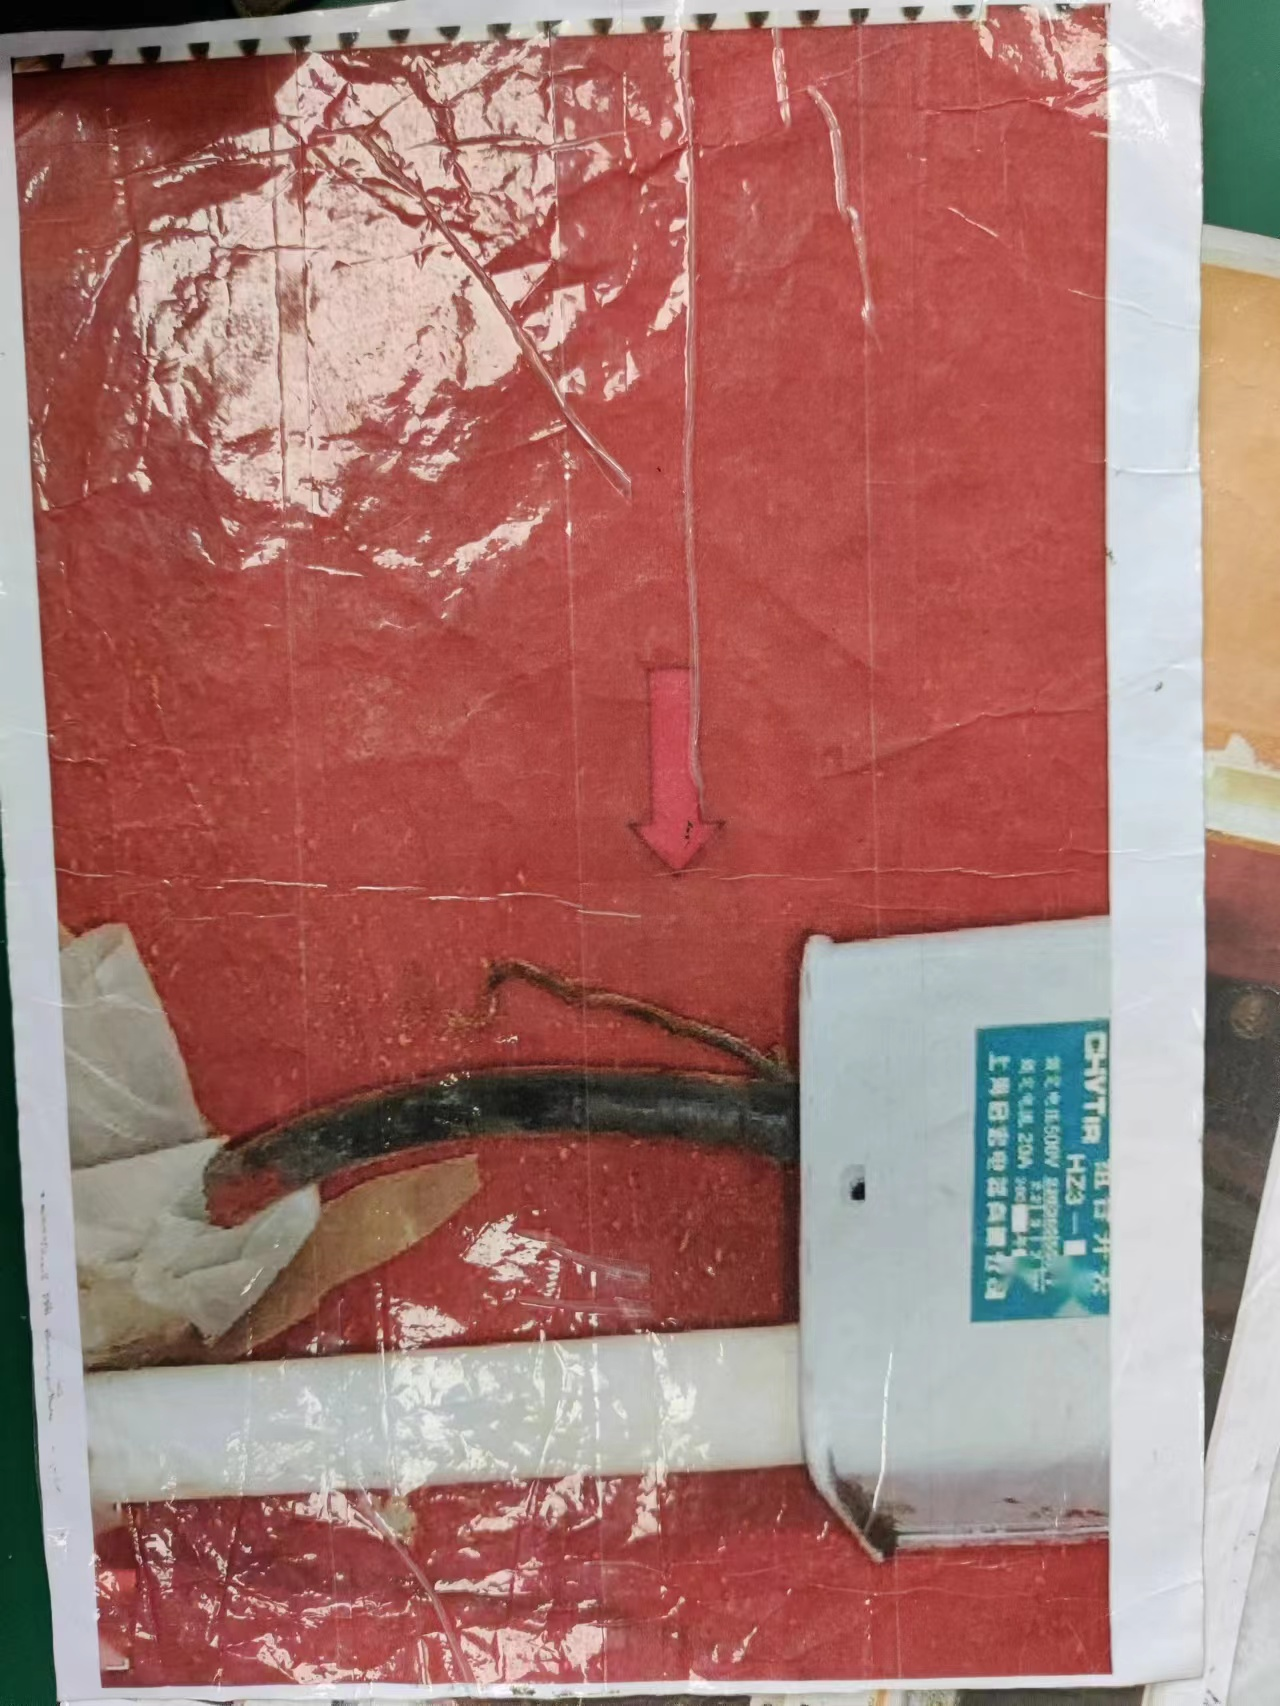
\includegraphics[width=0.55\textwidth]{1.jpg}}                        % fig1
				\caption*{\color{red}机器保护零线缺少}
				% \label{fig:example-a}
			\end{minipage}                       \hspace{2em}
			\begin{minipage}{0.45\textwidth}
				\centering
				\rotatebox{90}{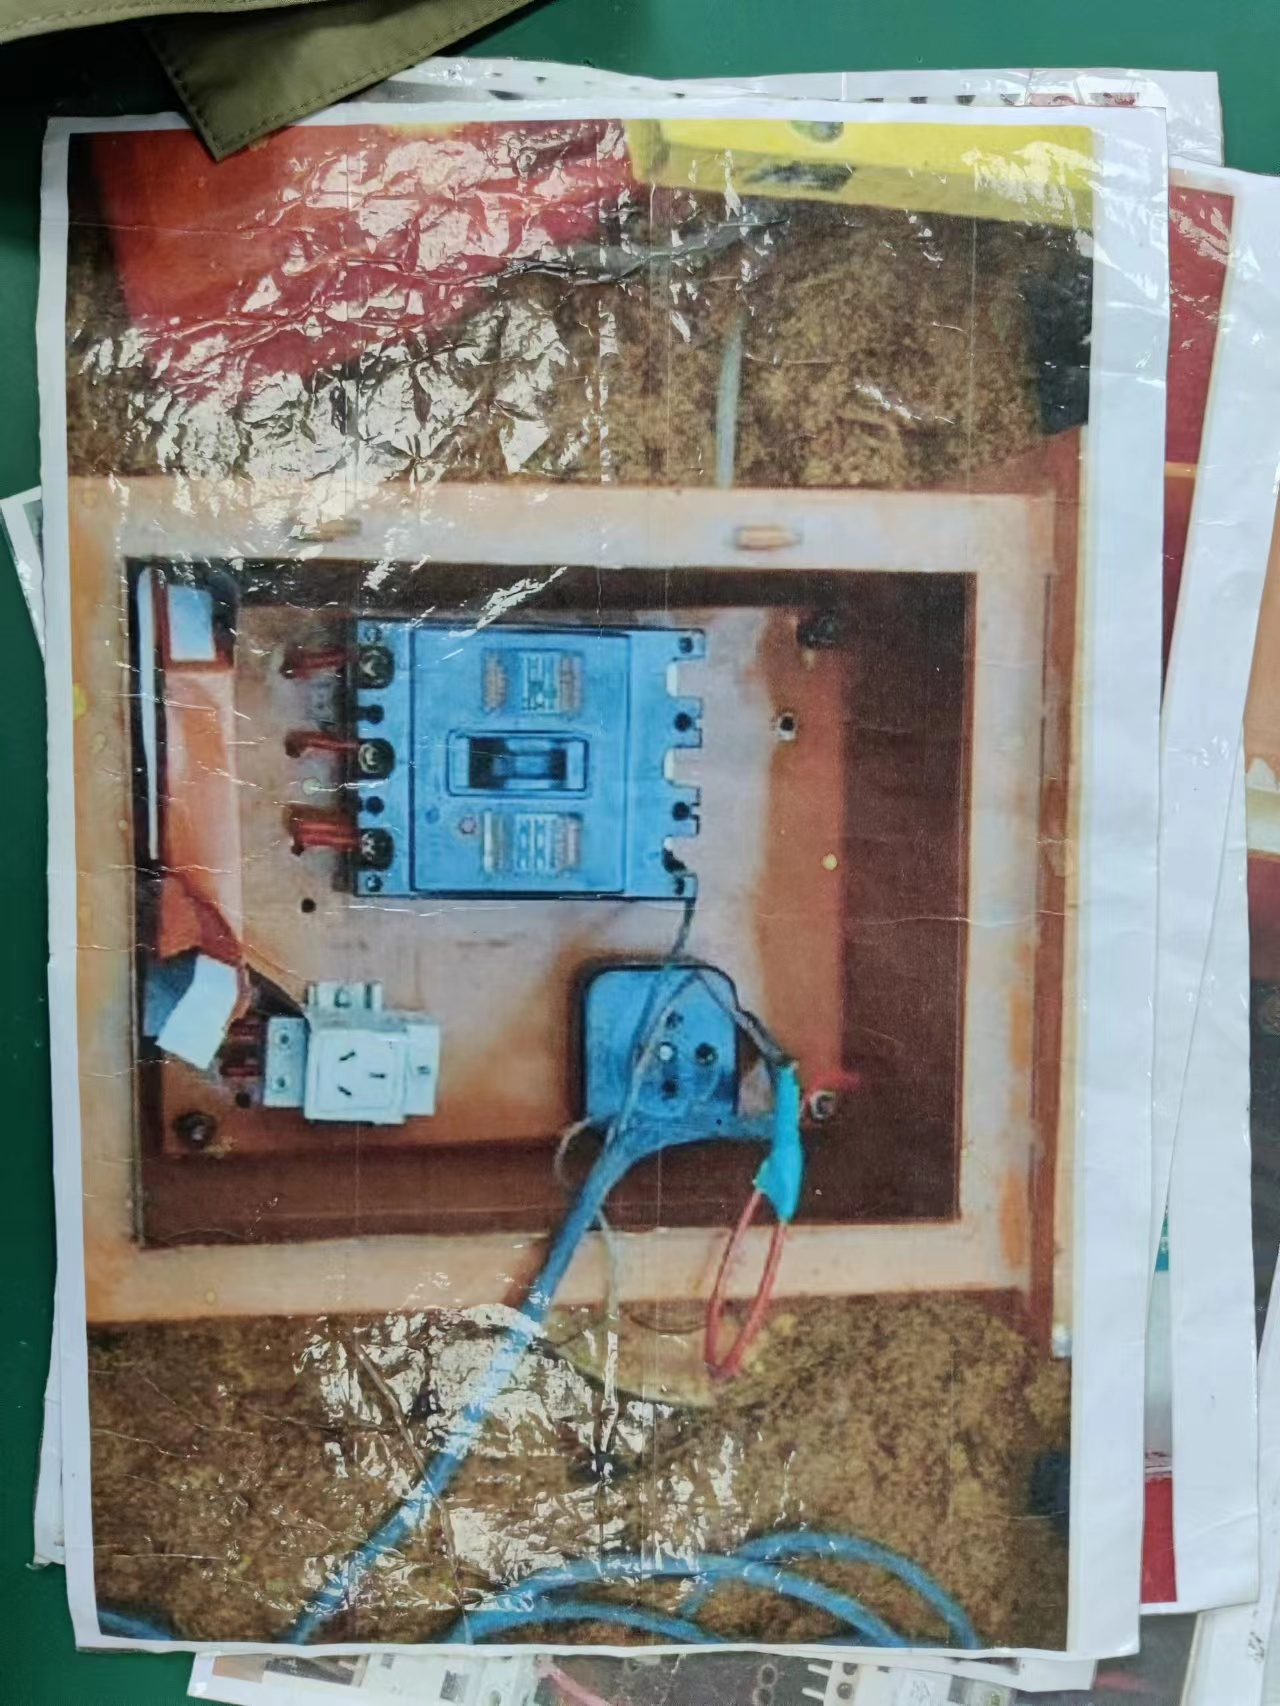
\includegraphics[width=0.55\textwidth]{2.jpg}}                     % fig2
				\caption*{电源进线不规范,动力照明混用}
				% \label{fig:example-b}
			\end{minipage}
		\end{figure}
		\vspace*{1cm}
				

		\begin{figure}[htbp]
			\centering
			\begin{minipage}{0.45\textwidth}
				\centering
				\rotatebox{90}{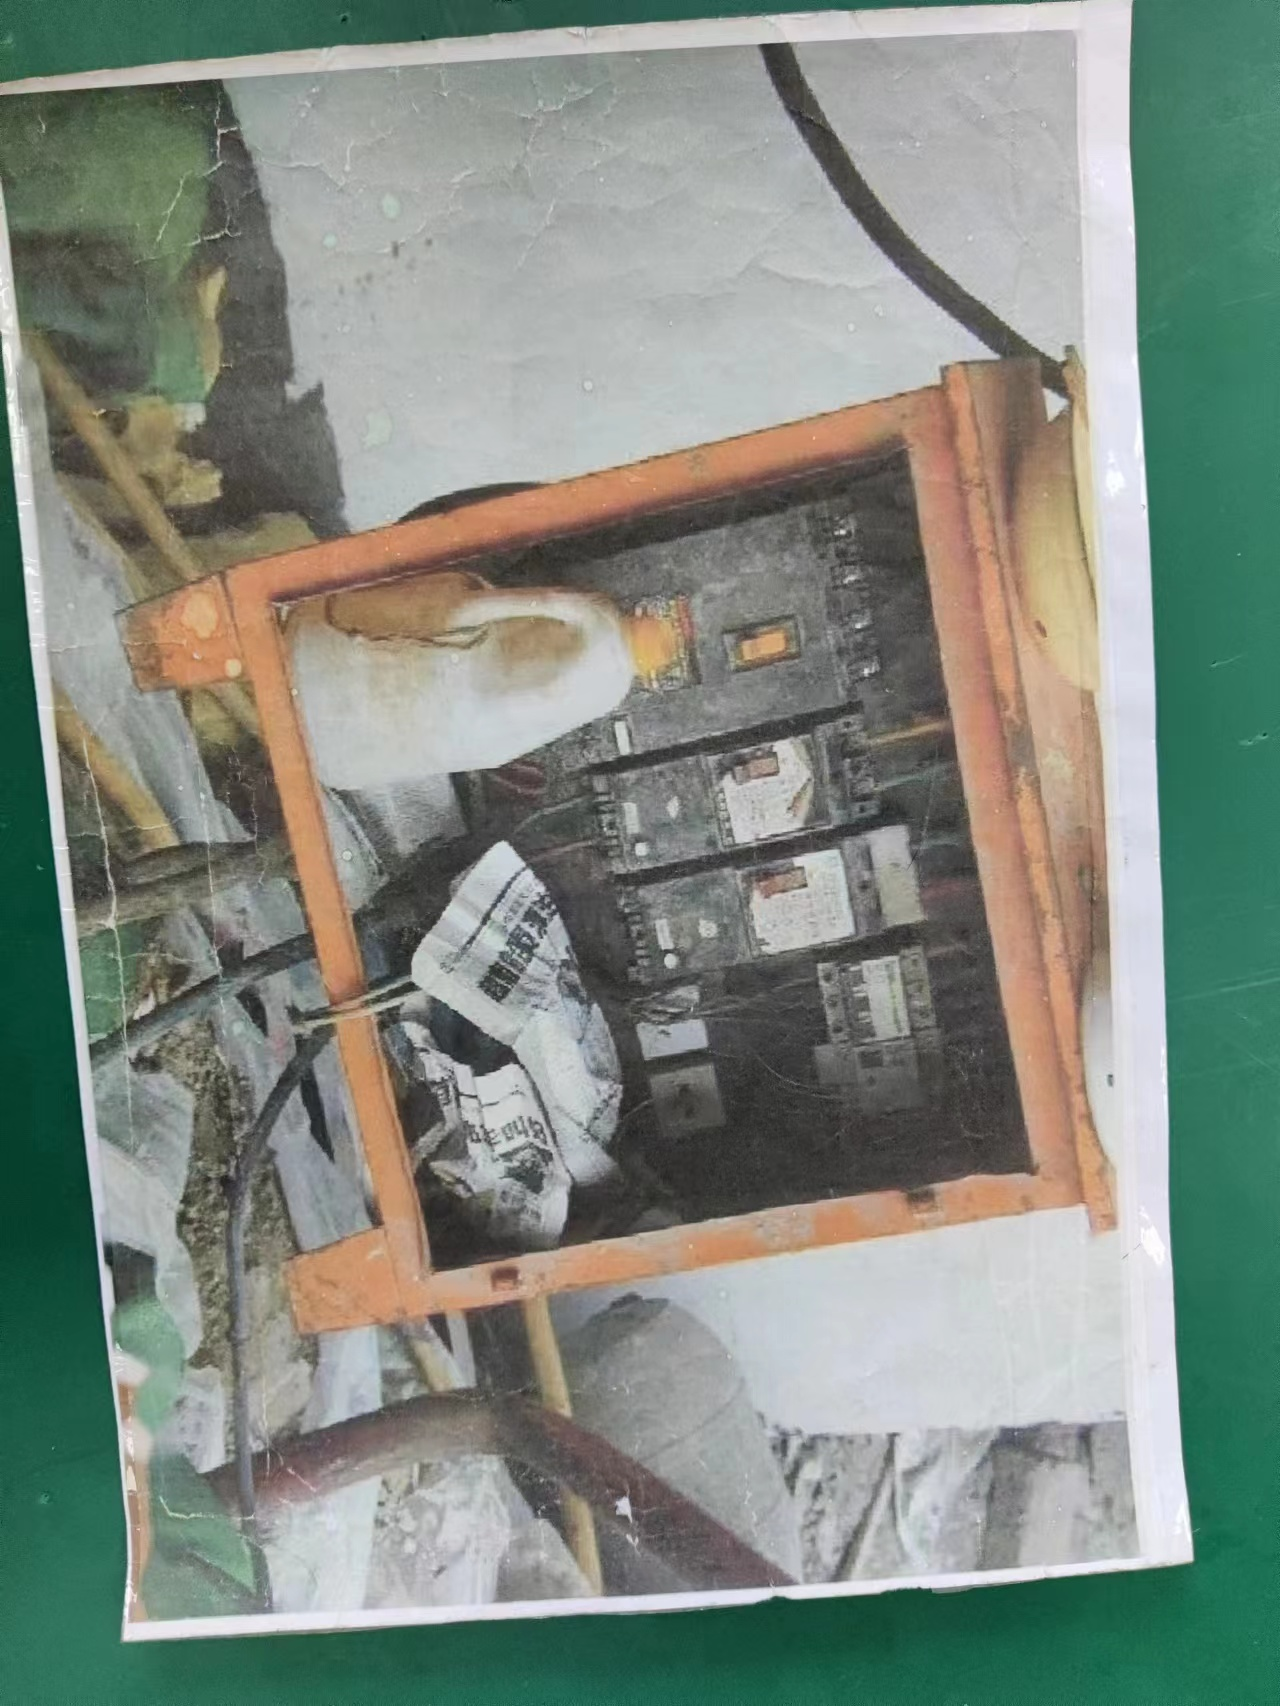
\includegraphics[width=0.55\textwidth]{3.jpg}}                      % fig3
				\caption*{配电箱内存放大量杂物,箱体无门,电器之间距离偏小,带电明露。}
						% \label{fig:example-a}
			\end{minipage}     \hspace{2em}
			\begin{minipage}{0.45\textwidth}
				\centering
				\rotatebox{90}{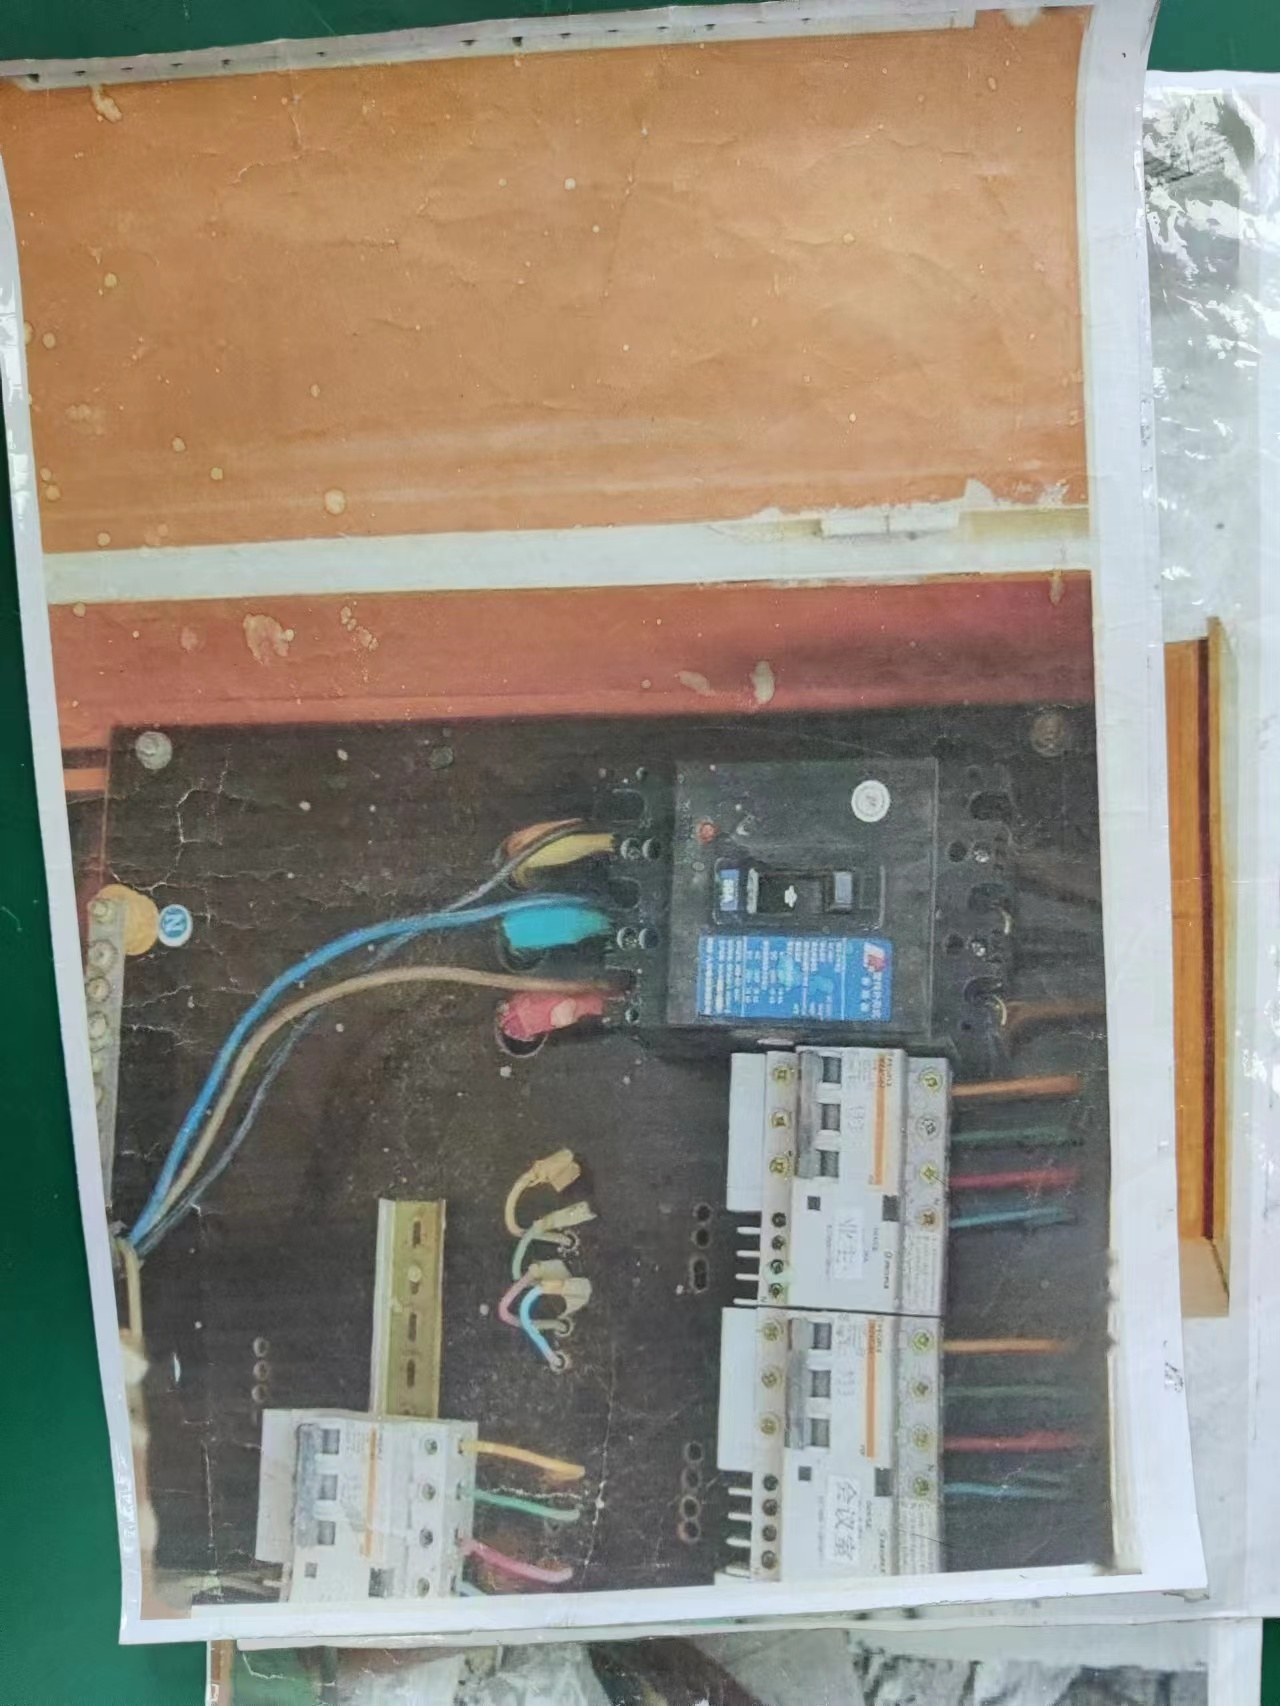
\includegraphics[width=0.55\textwidth]{4.jpg}}                    % fig4
				\caption*{违章从总空下口接线。}
						% \label{fig:example-b}
			\end{minipage}
		\end{figure}
		\vspace*{1cm}	
				

		\begin{figure}[htbp]
			\centering
			\begin{minipage}{0.45\textwidth}
				\centering
				\rotatebox{90} {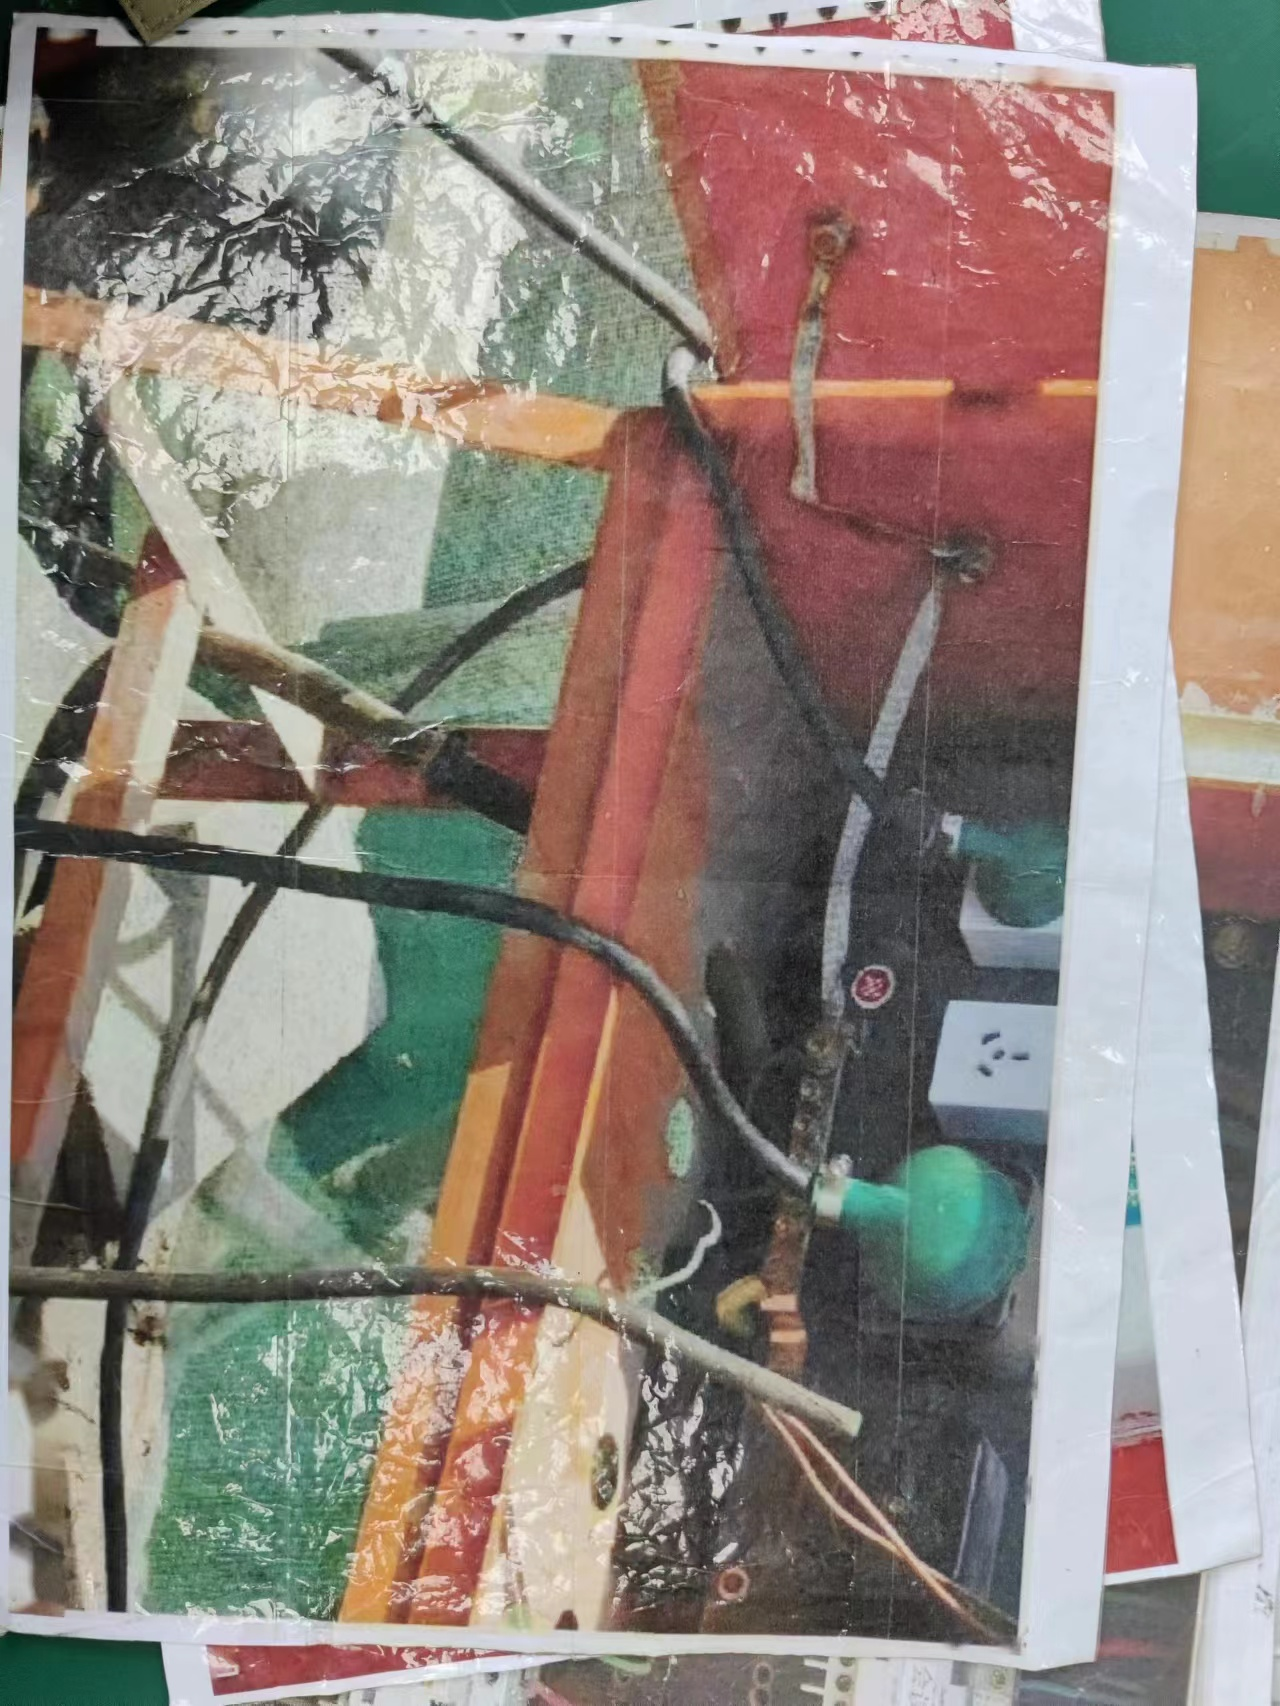
\includegraphics[width=0.55\textwidth]{5.jpg}}                   % fig5
				\caption*{电源出线从箱门位置出,容易夹断电缆发生事故。}
				% \label{fig:example-a}
			\end{minipage}     \hspace{2em}
			\begin{minipage}{0.45\textwidth}
				\centering
				\rotatebox{90}{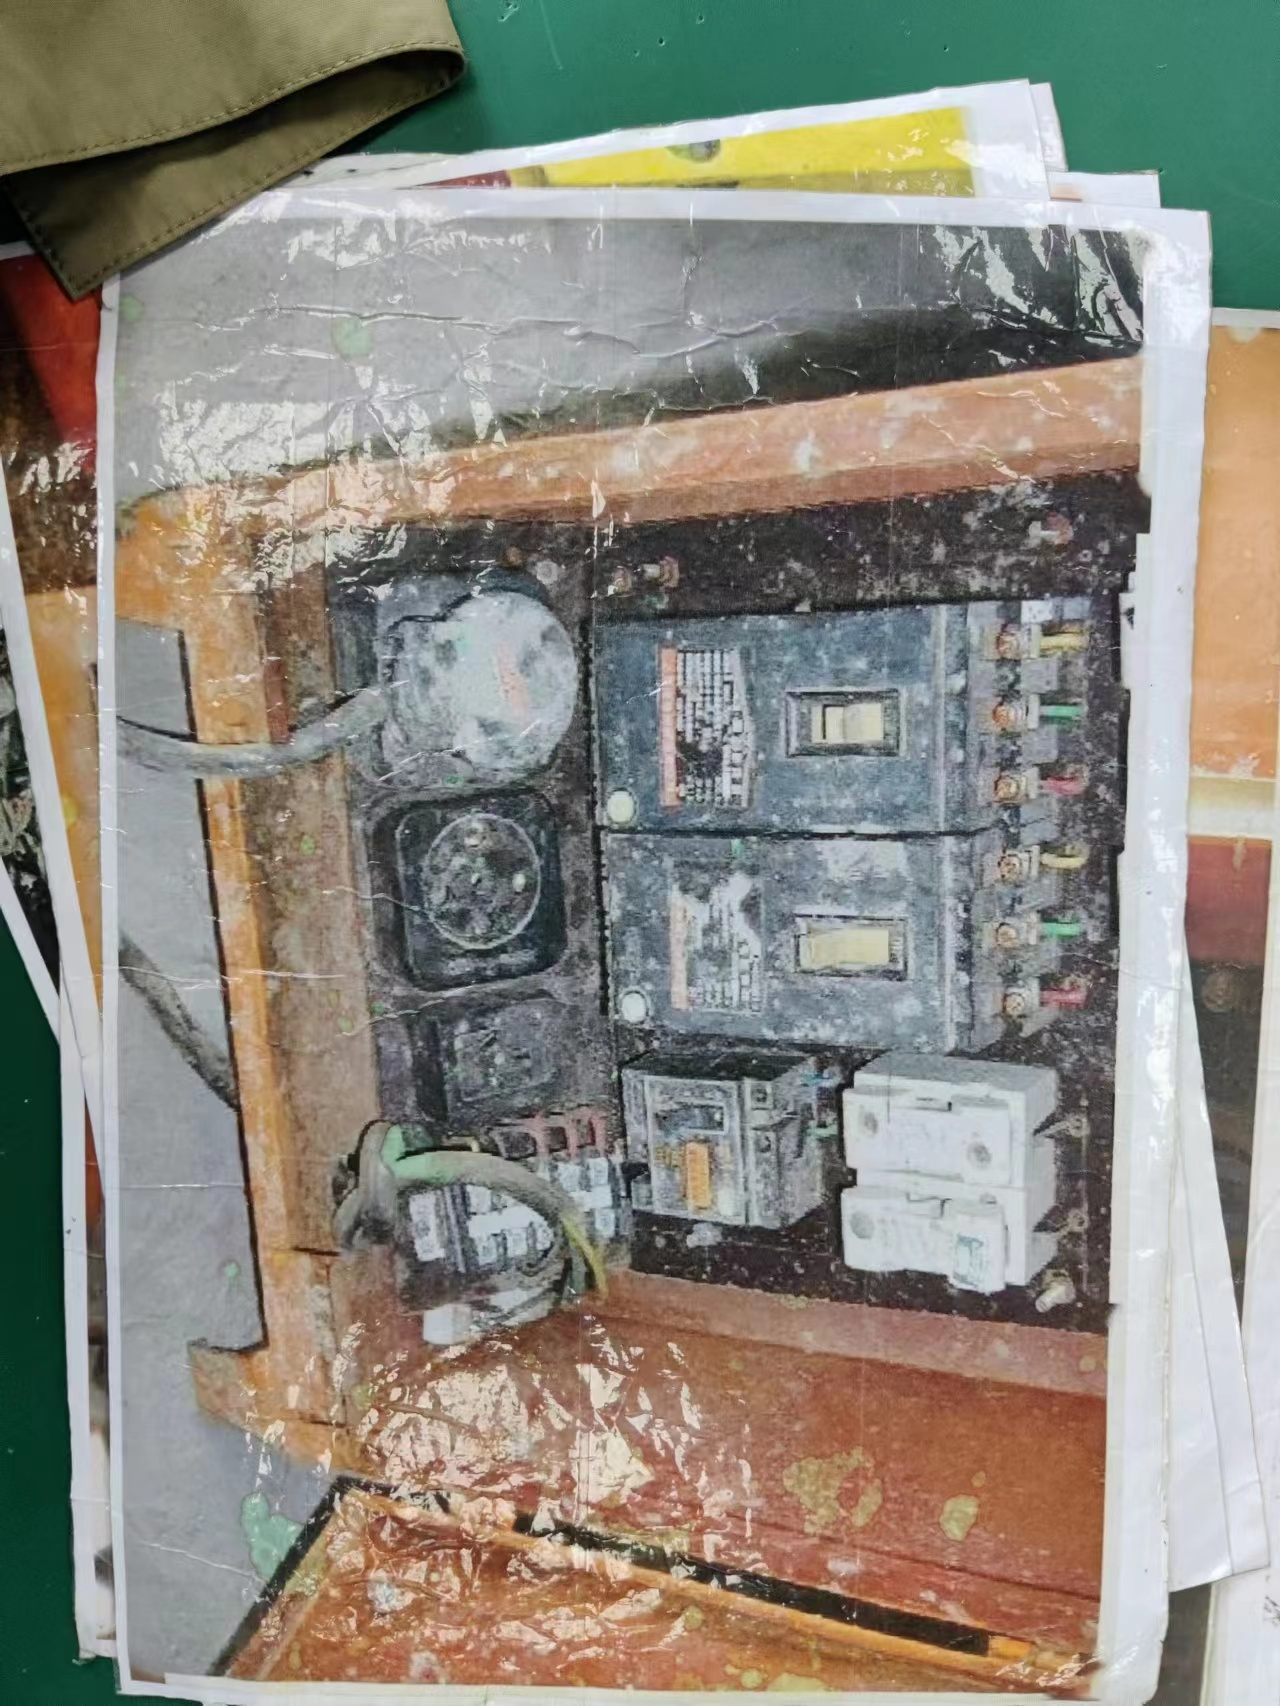
\includegraphics[width=0.55\textwidth]{6.jpg}  }                              % fig6
				\caption*{流动配电箱内存在火线接线端子板,带电明露}
				% \label{fig:example-b}
			\end{minipage}
		\end{figure}
		\vspace*{1cm}

		\begin{figure}[htbp]
			\centering
			\begin{minipage}{0.45\textwidth}
				\centering
				\rotatebox{90} {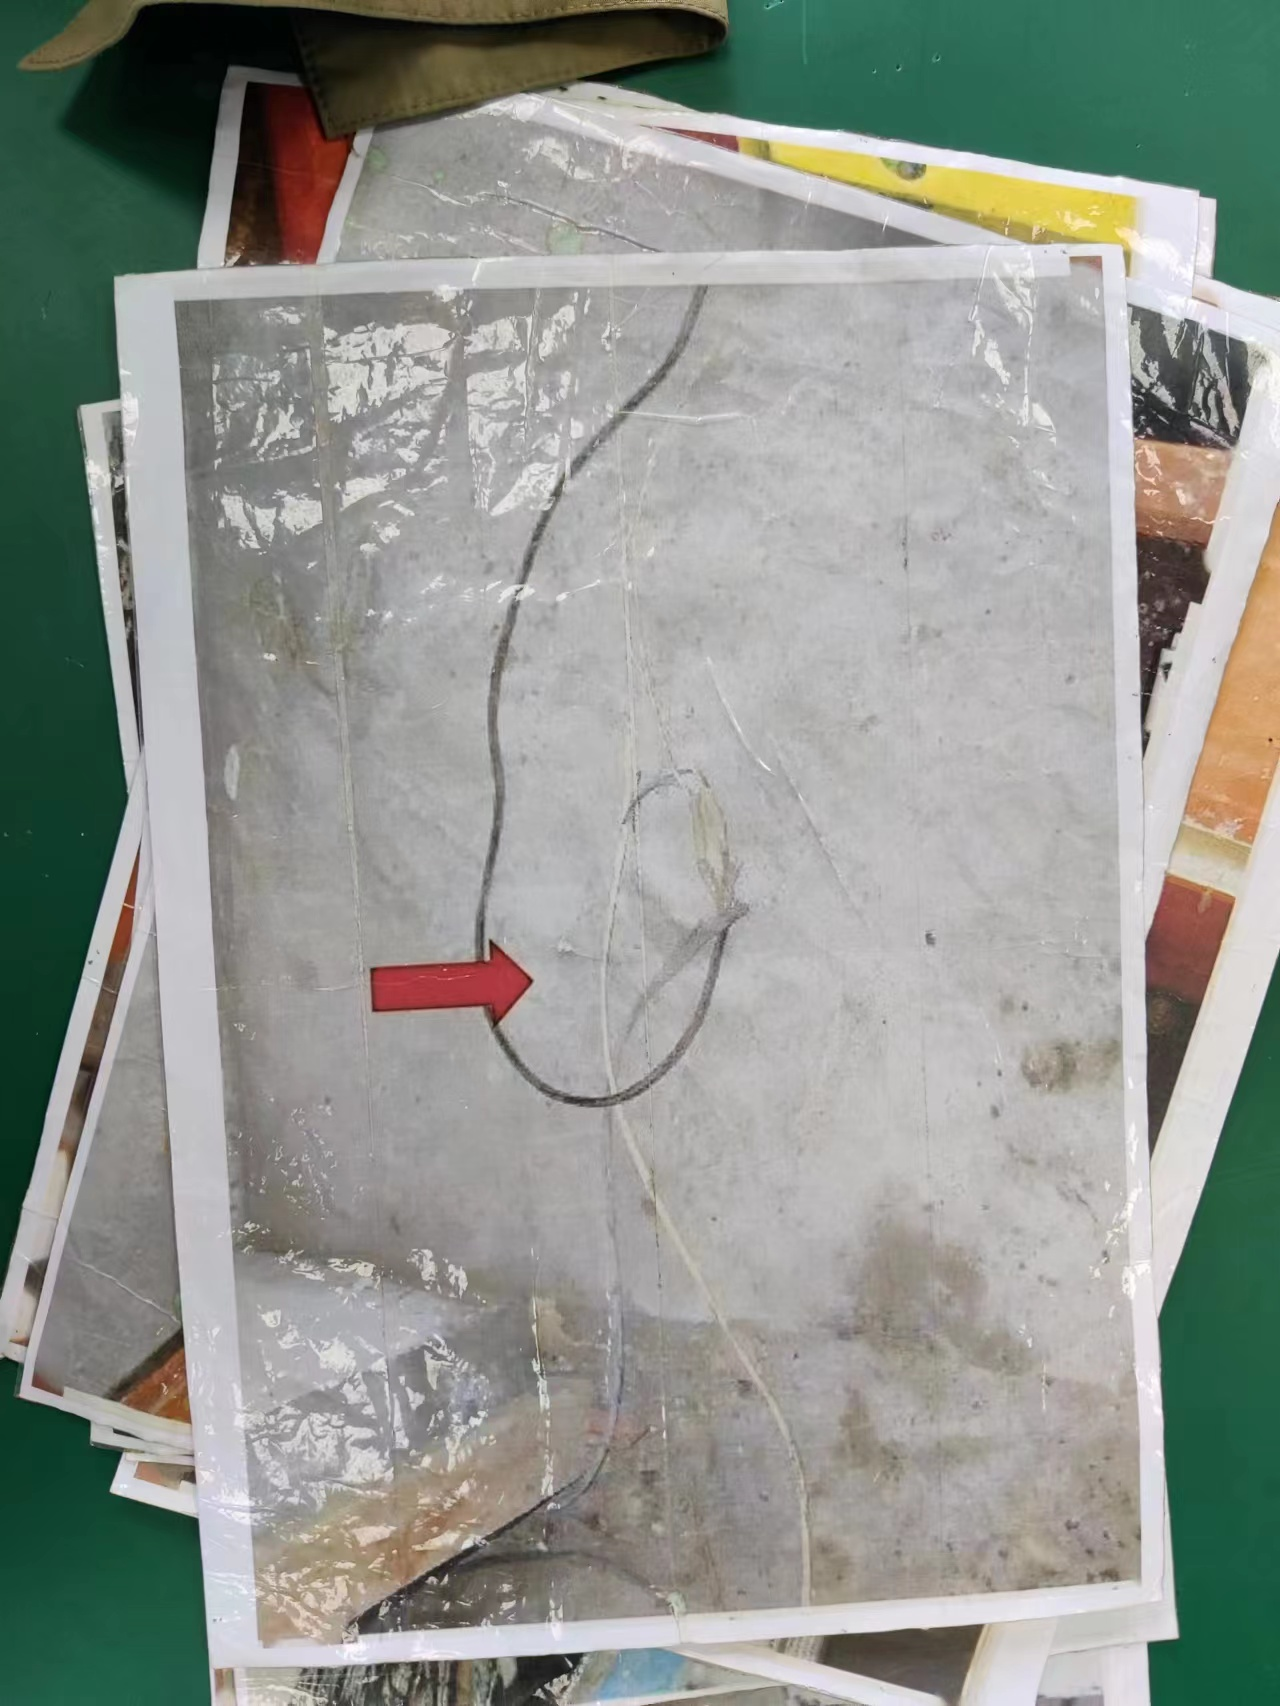
\includegraphics[width=0.55\textwidth]{7.jpg}}                   % fig7
				\caption*{电源线随意拖拉,街头处理过于简单。}
				% \label{fig:example-a}
			\end{minipage}     \hspace{2em}
			\begin{minipage}{0.45\textwidth}
				\centering
				\rotatebox{90}{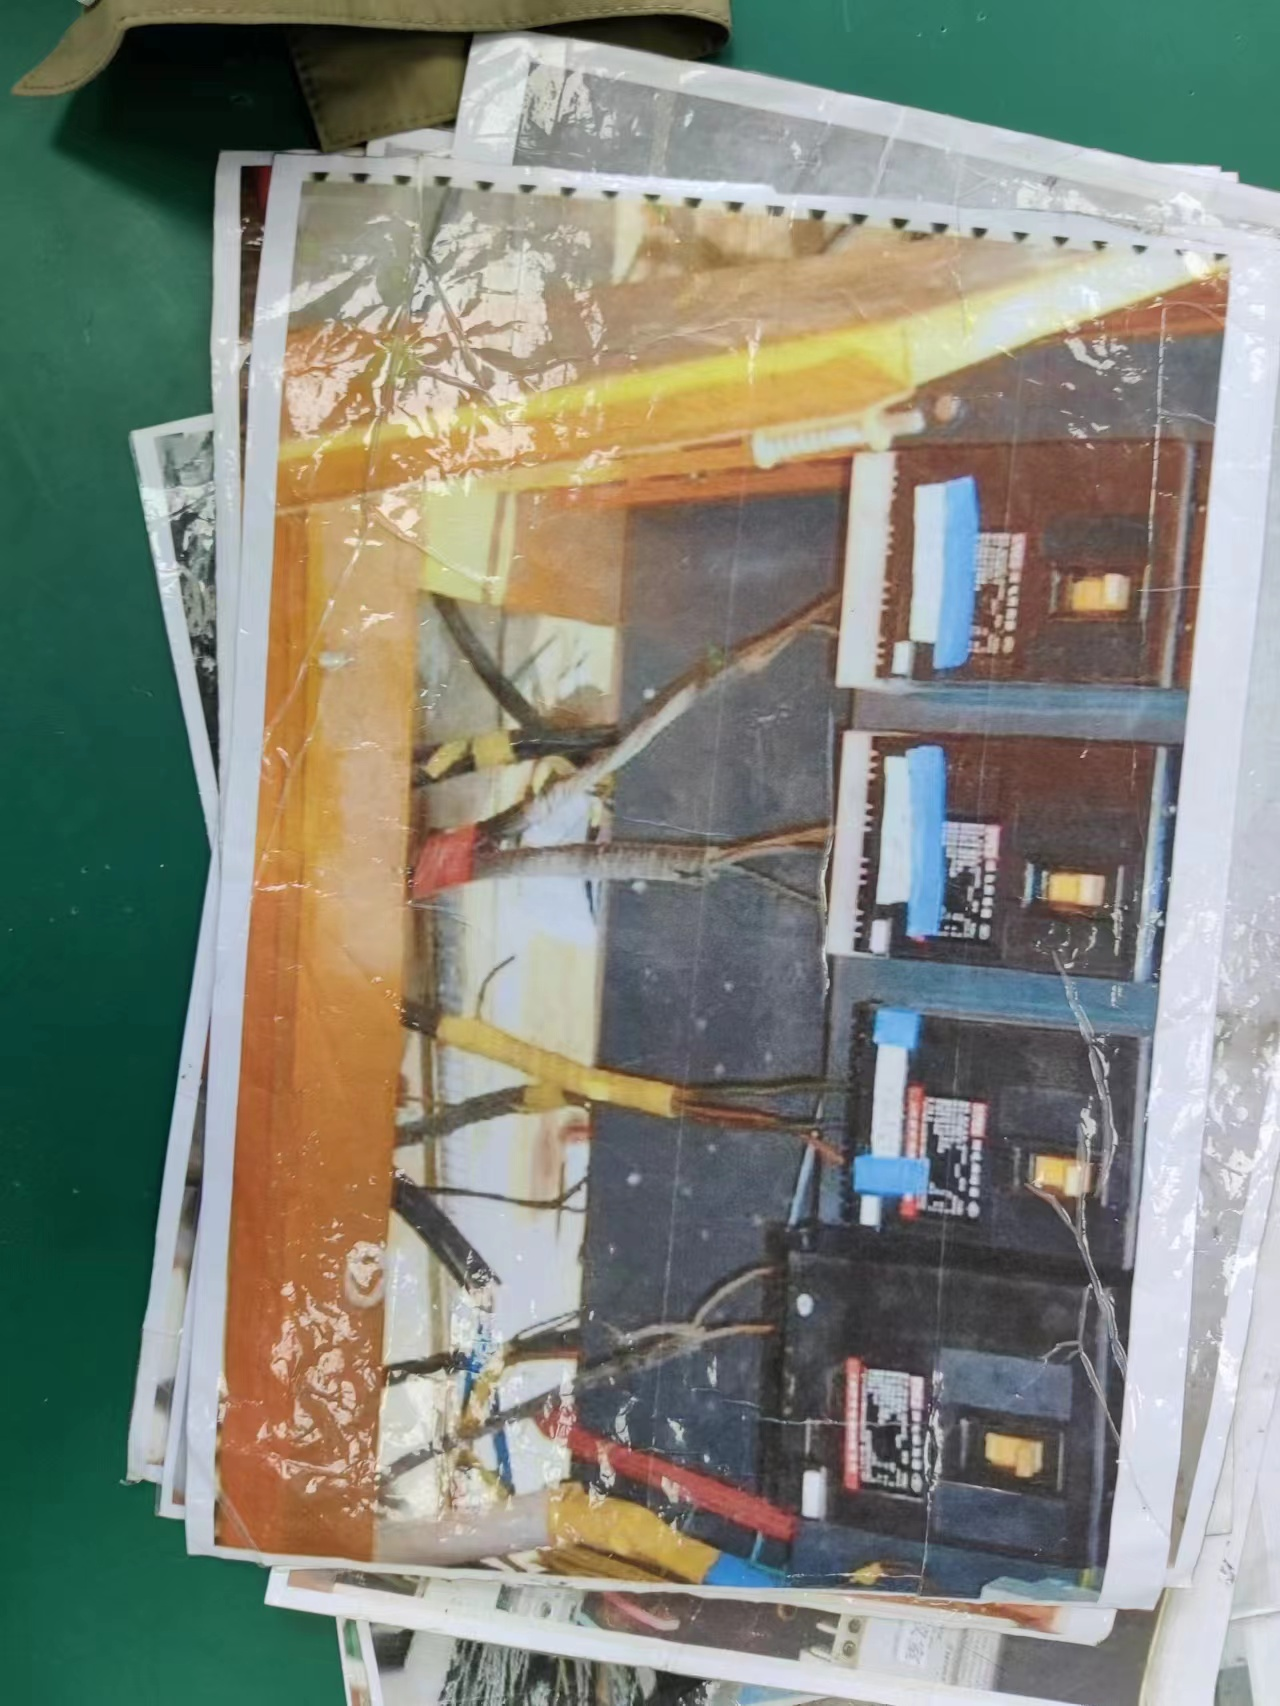
\includegraphics[width=0.55\textwidth]{8.jpg}  }                              % fig8
				\caption*{多台设备缺少保护零线。}
				% \label{fig:example-b}
			\end{minipage}
		\end{figure}
		\vspace*{1cm}
				

		\begin{figure}[htbp]
			\centering
			\begin{minipage}{0.45\textwidth}
				\centering
				\rotatebox{90} {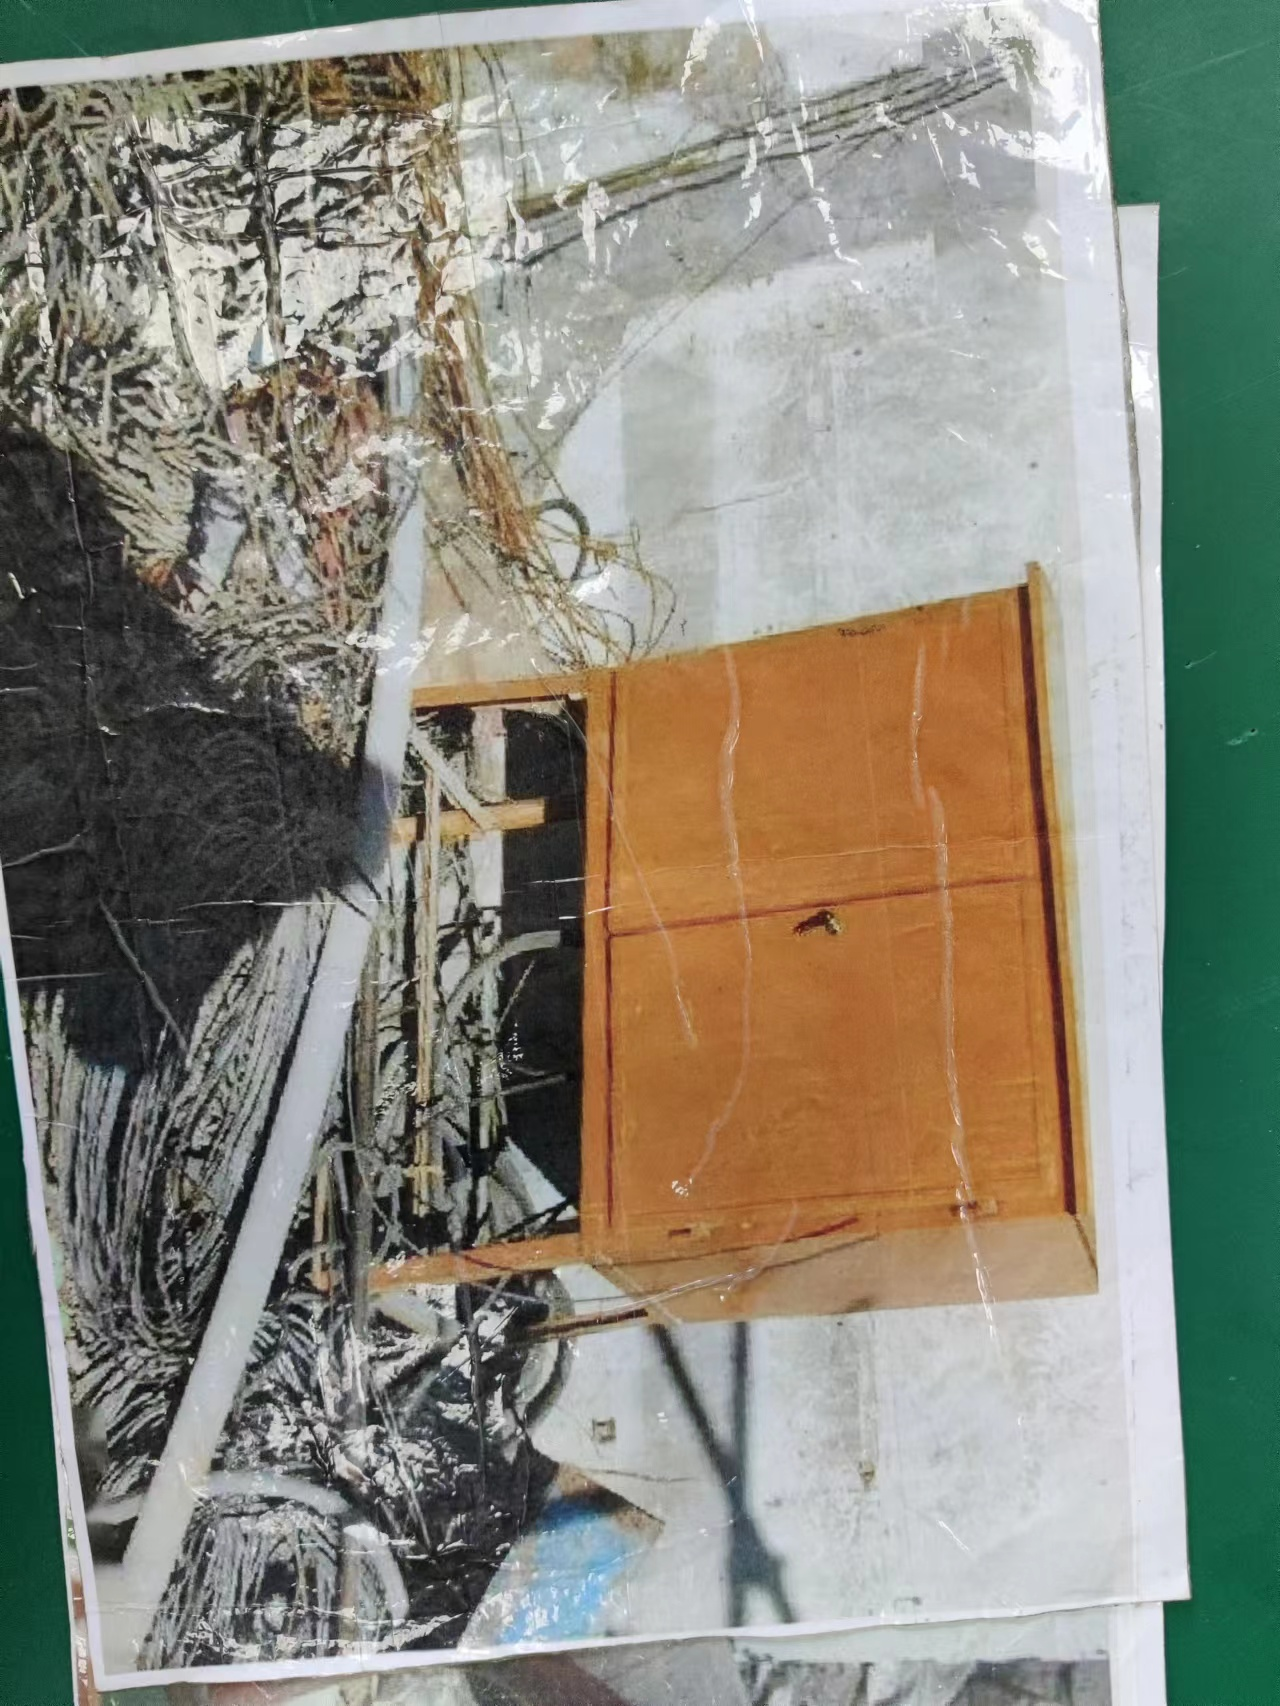
\includegraphics[width=0.55\textwidth]{9.jpg}}                   % fig9
				\caption*{配电箱附近堆积大量金属杂物,电缆缺少保护措施,缺少防触电标志、负责人。}
				% \label{fig:example-a}
			\end{minipage}     \hspace{2em}
			\begin{minipage}{0.45\textwidth}
				\centering
				\rotatebox{90}{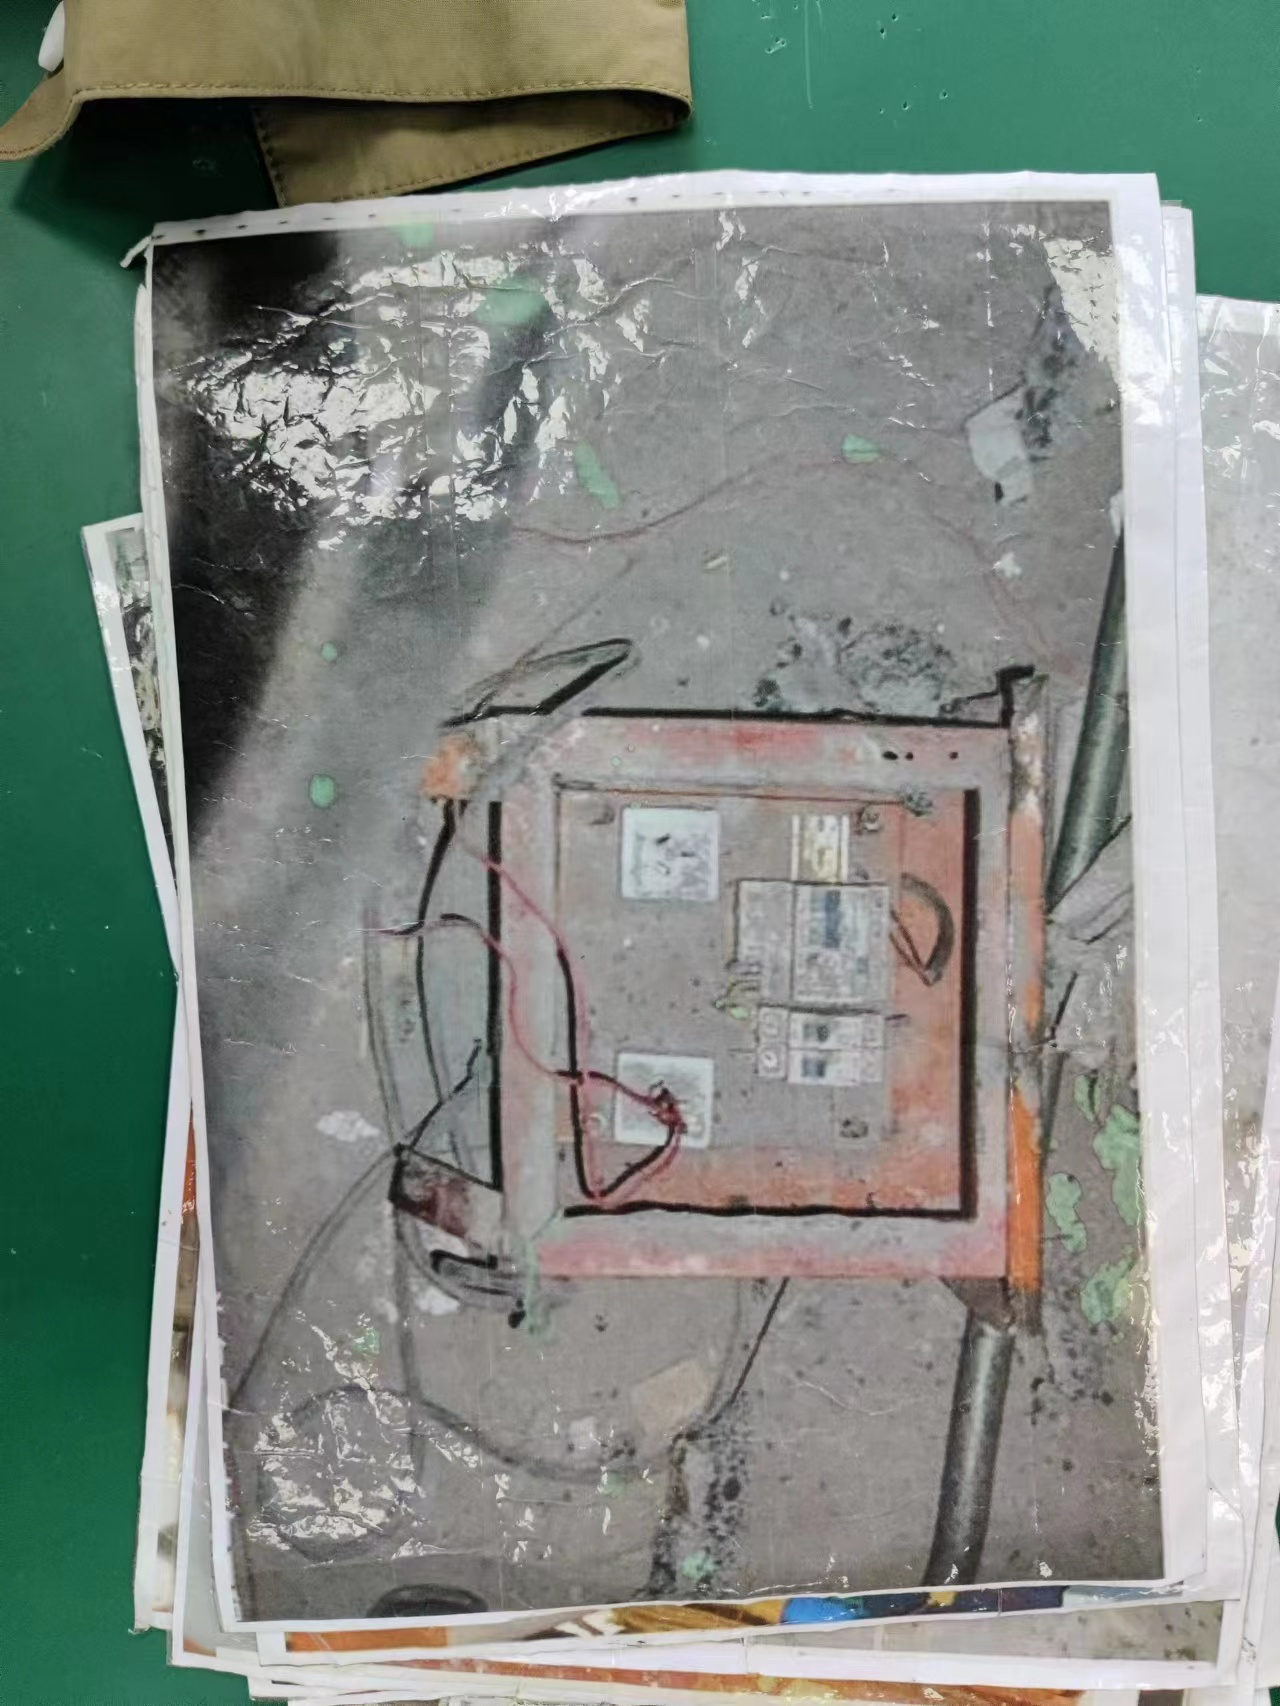
\includegraphics[width=0.55\textwidth]{10.jpg}  }                              % fig10
				\caption*{电闸箱无门、倒放。}
				% \label{fig:example-b}
			\end{minipage}
		\end{figure}
		\vspace*{1cm}


		\begin{figure}[htbp]
			\centering
				\rotatebox{90} {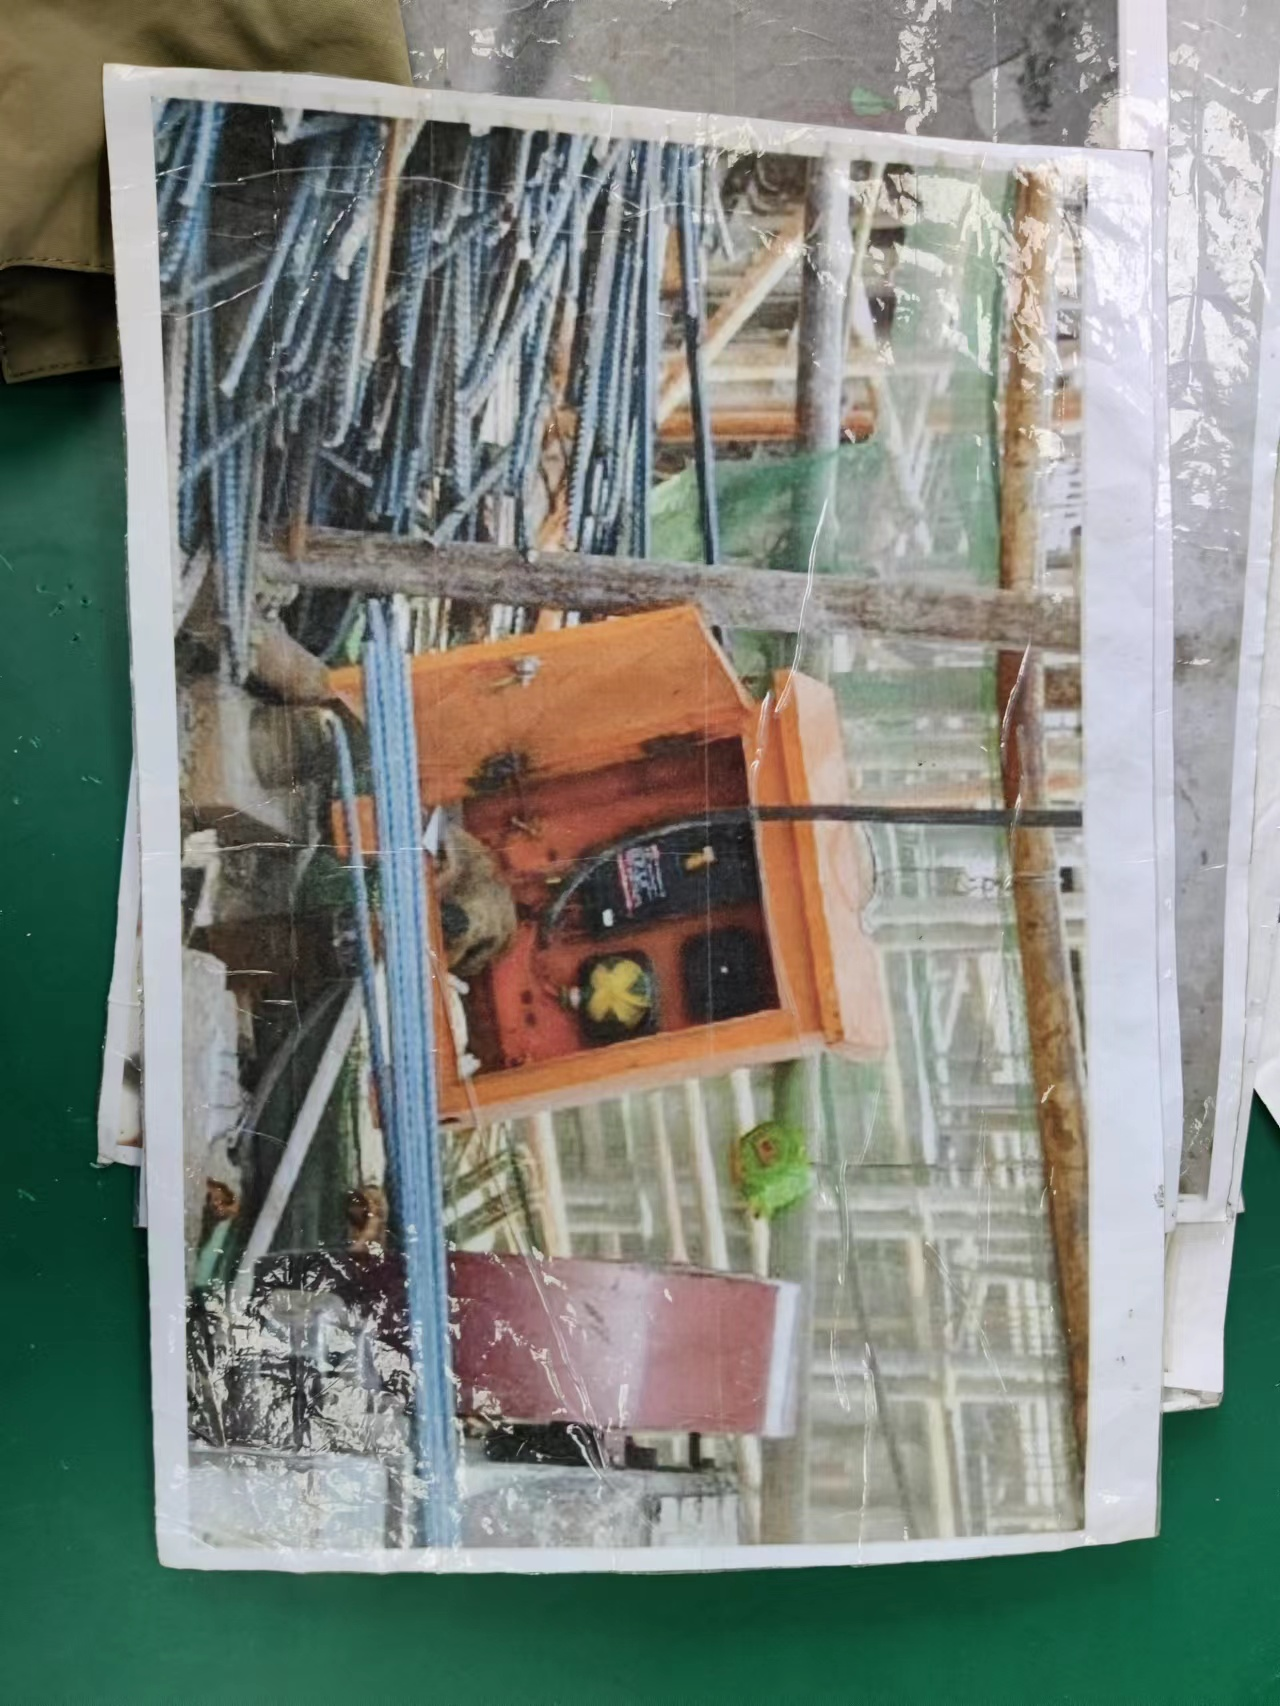
\includegraphics[width=0.2475\textwidth]{11.jpg}}                   % fig11
				\caption*{设备专用开关箱安装位置距地面距离偏小,且箱内存放杂物,一闸多机等。}
		\end{figure}
		\vspace*{1cm}
%%%%%%%%%%%%%%%%%%%%%%%%%%%%%%%%%%%%%%%%%%%
		\begin{figure}[htbp]
			\centering
			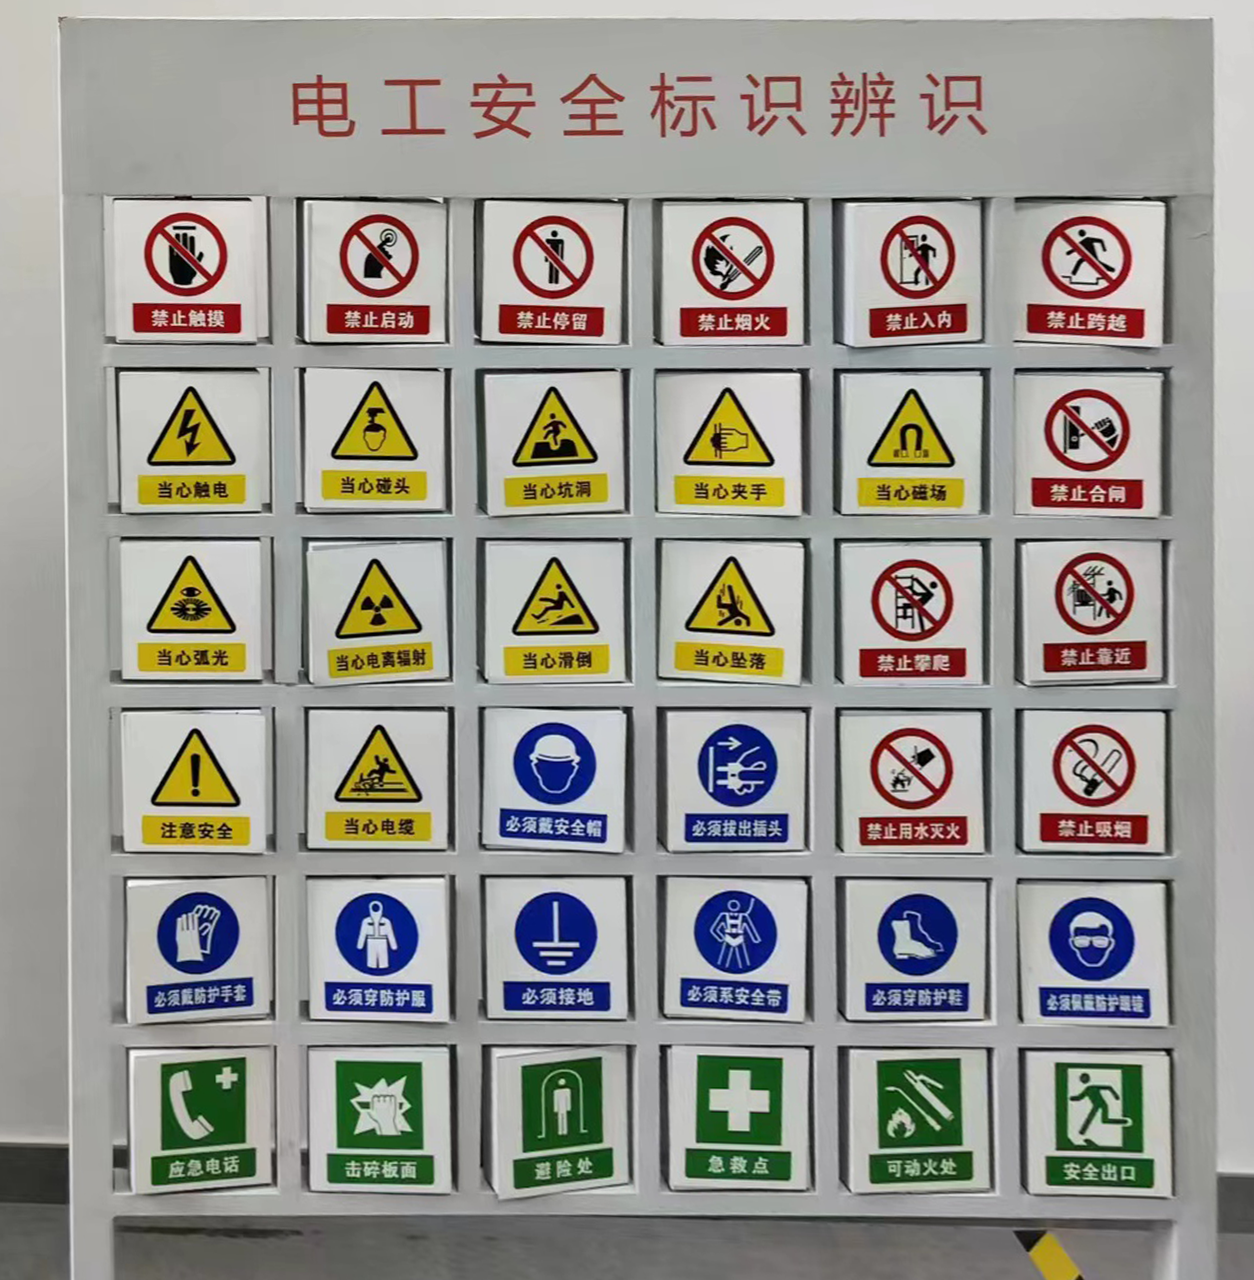
\includegraphics[width=0.9\textwidth]{125.png}
			\caption*{记住所有的符号。}
		\end{figure}

		% \begin{figure}[htbp]
		% 	\centering
		% 	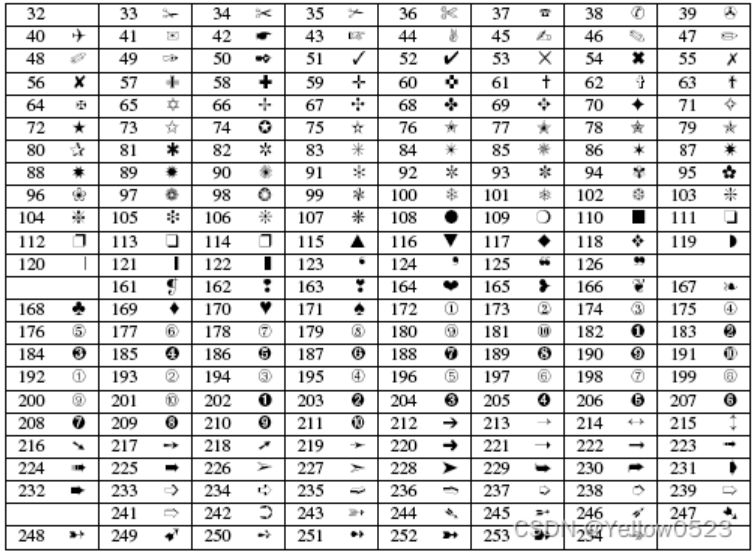
\includegraphics[width=0.9\textwidth]{pifont.png}
		% 	\caption*{对照表。}
		% \end{figure}










